\documentclass[First Project.tex]{subfiles}

\begin{document}
\subsection{ Βελτίωση του βαθμού σημαντικότητας μίας σελίδας }

Σε αυτή την παράγραφο προσθέτονται 4 συνδέσεις και αφαιρείται 1 από το υποθετικό μας δίκτυο με σκοπό να βελτιωθεί ο βαθμός σημαντικότητας της
σελίδας 1. Για να το πετύχουμε αυτό αφαιρούμε την σύνδεση \textbf{(10,13)} ώστε να μην μεταφέρεται
η σημαντικότητα της σελίδας 10 στην σελίδα 13. Έπειτα, προσθέτουμε τις συνδέσεις \textbf{(10,1)},\textbf{(11,1)},
\textbf{(15,11)} και \textbf{(11,10)} ώστε να μεταφέρουμε την σημαντικότητα των σελίδων 10 και 11, που έχουν 
τον μεγαλύτερο βαθμό εισόδου, στην σελίδα 1. Οι υπόλοιπες σελίδες έχουν βαθμό εισόδου 2 επομένως επιλέγουμε την σελίδα 15 να δείχνει στην 1
καθώς η σελίδα 15 είναι η μόνη που δείχνει η 11, με την 11 να είναι μία από τις δύο σελίδες με τον μεγαλύτερο βαθμό εισόδου. Η στρατηγική αυτή 
είναι η κεντρική ιδέα πίσω από το \textlatin{\textbf{google-bombing}}, όπου σκοπός είναι η αύξηση του βαθμού σημαντικότητας μιας 
ιστοσελίδας πείθοντας άλλες ιστοσελίδες με υψηλή κίνηση (\textlatin{\textbf{high-traffic}}) να δείχνουν σε αυτή.

\begin{figure}[h!]
    \centering
    \captionsetup{justification=centering}
    \begin{center}
        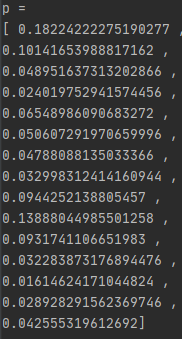
\includegraphics[scale=0.65]{exercise_4_modified_network.png}    
        \caption{ Τάξη των σελίδων του υποθετικού δικτύου μετά τις προσθαφαιρέσεις συνδέσεων για να βελτιωθεί 
        ο βαθμός σημαντικότητας της σελίδας 1 }
    \end{center}
\end{figure} 

Οι νέες τάξεις σελίδας μετά τις τροποποιήσεις των συνδέσεων φαίνονται στο \textit{Σχήμα 51}, όπου παρατηρούμε ότι καταφέραμε με την χρήση μιας
στρατηγικής παρόμοιας με το \textlatin{\textbf{google-bombing}} να βελτιώσουμε τον βαθμό σημαντικότητας της σελίδας 1.
\end{document}